\lecture{Recuperação de Portadora}{lec_carrier}

\begin{frame}
	\begin{block}{\centering\large\bfseries Parte 6}
		\centering\large\insertpart
	\end{block}
\end{frame}

\section{Introdução}
\begin{frame}
	\frametitle{Introdução}
	
	Os sinais transmitidos estão sujeitos a desvios em frequência e em fase devido aos seguintes fatores:
	
	\begin{itemize}
		\item \textbf{Desvio em Frequência}: Causado por instabilidades no oscilador do transmissor ou receptor e pelo efeito Doppler quando o receptor está se locomovendo em relação ao transmissor.
		
		\item \textbf{Desvio em Fase}: Devido à instabilidade de fase dos osciladores, a atrasos de transmissão e ao ruído térmico. 
	\end{itemize}
	
	Nesta aula analisaremos formas de estimar e corrigir os devios nos sinais recebidos. 
\end{frame}

\begin{frame}
	\frametitle{Introdução}
	\begin{itemize}		
	
		\item Considere o Sinal PAM sujeito a desvio de frequência ou \textit{jitter} em fase modelados como $\theta(t)$:
		\begin{equation*}
			e^{j(2\pi f_c + \theta(t))}\sum_{m=-\infty}^{\infty}A_m p(t-mT)
		\end{equation*}
		
		
		
		\item Uma portadora com estimativa de fase $\phi(t)$ é usada para a demodulação
		\begin{equation*}
			e^{-j(2\pi f_c + \phi(t))}
		\end{equation*}
		
		\item O sinal é demodulado e amostrado com taxa $t=kT$, considerando que a formatação de pulso satisfaz o critério de Nyquist $(p_k=\delta_k)$
		
		%q_k=e^{j(\theta_k - \phi_k)}\sum_{m=-\infty}^{\infty}A_k
		\begin{equation*}
			q_k=e^{j(\theta_k - \phi_k)}A_k
		\end{equation*}
	\end{itemize}
	
\end{frame}

\begin{frame}
	\frametitle{Introdução}
	\begin{itemize}
		\item Com um erro de fase constante $(\theta_k - \phi_k=\Psi)$ a constelação recebida será uma versão inclinada da real:
		\begin{figure}
			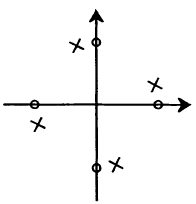
\includegraphics[width=0.2\columnwidth]{figs/inclidado}
		\end{figure}
		
		\item Com um erro de frequência $(\theta_k - \phi_k=2\pi f_0 k T)$ a constelação recebida rotaciona:
		
		\begin{figure}
			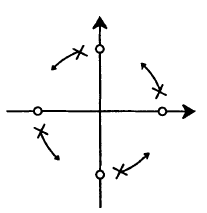
\includegraphics[width=0.2\columnwidth]{figs/rotacionando}
		\end{figure}
	\end{itemize}
	
\end{frame}

\section{Recuperação Direcionada a Decisão}

\begin{frame}
	\frametitle{Recuperação Direcionada a Decisão}
	\begin{itemize}
		
		\item A partir do sinal demodulado $q_k$ é possível encontrar uma estimativa do erro de fase:
		\begin{equation*}
			\varepsilon_k=\theta_k - \phi_k= \sin^{-1}\biggl(\frac{\operatorname{Im}\{q_k A_k^*\}}{|A_k|^2}\biggr)
		\end{equation*}
		
		\item Porém os simbolos $A_k$ não são conhecidos nos receptores.
		\item Usaremos as decisões $\hat{A}_k$ ao invés dos símbolos reais. 
		
		\begin{figure}
			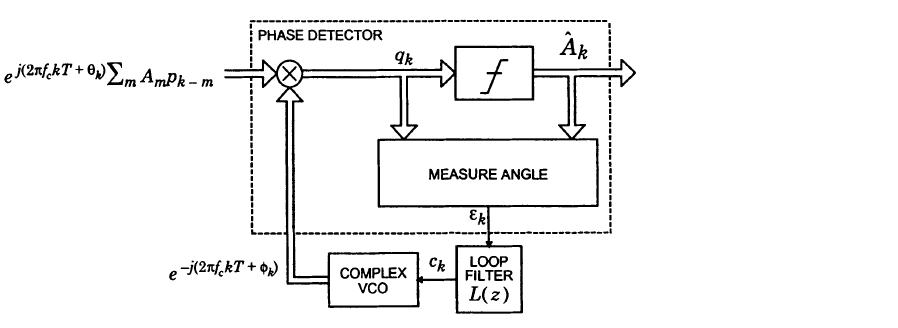
\includegraphics[width=0.9\columnwidth]{figs/DDPLL}
		\end{figure}

	\end{itemize}
	
\end{frame}


\begin{frame}
	\frametitle{Recuperação Direcionada a Decisão}
	\begin{itemize}
		
		\item Em um sinal 4-PSK com erros maiores que $\pi/4$ a decisão será incorreta:
		
		\begin{figure}
			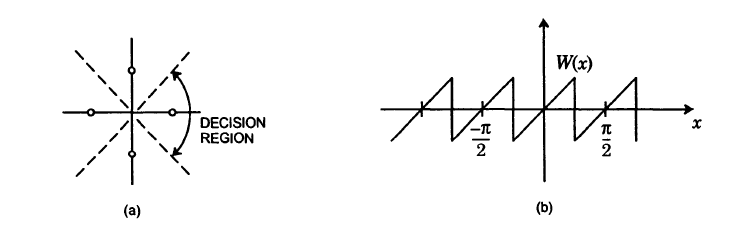
\includegraphics[width=0.8\columnwidth]{figs/4psk}
		\end{figure}
		
		\item Este erro de decisão é chamado de ambiguidade de fase.
		
		\item Para corrigí-lo pode ser utilizado um codificador diferencial.
		\begin{figure}
			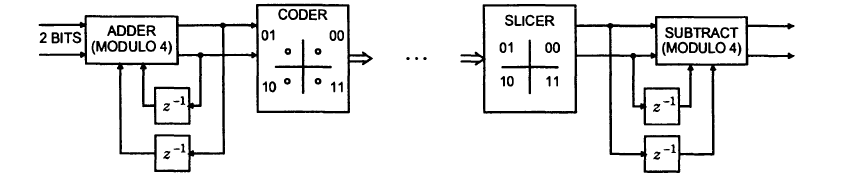
\includegraphics[width=0.9\columnwidth]{figs/coddif}
		\end{figure}
		
	\end{itemize}
	
\end{frame}



\begin{frame}
	\frametitle{Recuperação Direcionada a Decisão}
	\begin{itemize}
		
		\item A expressão do erro de fase pode ser simplificada. Para erros de fase pequenos $\varepsilon_k=\sin(\varepsilon_k)$ e
		\vspace{-3.5ex}
		\begin{columns}
			\begin{column}{0.5\linewidth}
				\begin{equation*}
					\sin(\varepsilon_k)=\frac{\operatorname{Im}\{q_k A_k^*\}}{|A_k|^2}= W'
				\end{equation*}
			\end{column}
			\begin{column}{0.5\linewidth}
				\begin{figure}
					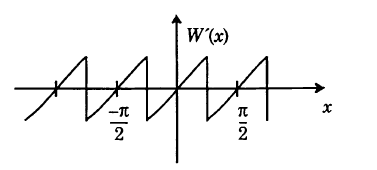
\includegraphics[width=0.7\columnwidth]{figs/fasedetec}
				\end{figure}
			\end{column}
		\end{columns}

		\item Ou ainda mais simplificado (comumente utilizado): $\varepsilon'_k=\operatorname{Im}\{q_k A_k^*\}$		
% 		\vspace{-3ex}
		\begin{figure}
			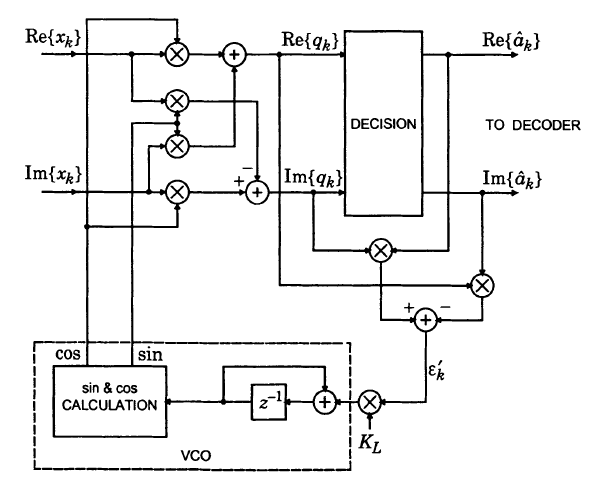
\includegraphics[width=0.45\columnwidth]{figs/realdd}
		\end{figure}
			
	\end{itemize}
\end{frame}


\section{Potência de $N$}

\begin{frame}
	\frametitle{Potência de $N$}
	\begin{itemize}
		
		\item Em situações com baixa SNR a Recuperação Direcionada a Decisão apresenta muitos erros.
		
		\item O método da potência de N pode ser utilizado como uma alternativa.
		
		\item Considere novamente um sinal amostrado PAM 
			\begin{equation*}
			x_k=e^{j(2\pi f_ckT +\theta_k)}\sum_{m=-\infty}^{\infty}|A_m|e^{j\phase A_m}p_{k-m}
			\end{equation*}
		\item Considere ISI nula $(p_k=\delta_k)$
		\begin{equation*}
		x_k=e^{j(2\pi f_ckT +\theta_k)}|A_k|e^{j\phase A_k}
		\end{equation*}
		
		\item Se elevássemos os dois lados à $N$-ésima potência e supondo que existe um $N$ tal qual $e^{jN \phase A_k}=1$
		\begin{equation*}
		x_{k}^N=e^{jN(2\pi f_ckT +\theta_k)}|A_k|^N
		\end{equation*}
			
	\end{itemize}
	
\end{frame}

\begin{frame}
	\frametitle{Potência de $N$}
	\begin{itemize}
		
		\item Este sinal tem uma forte linha espectral em $N f_c$ que pode ser extraída utilizando um filtro passa banda
% 		\begin{equation*}
% 		x_{k}^N=e^{jN(2\pi f_ckT +\theta_k)}|A_m|^N
% 		\end{equation*}
		\begin{equation*}
		x_{k}^N=e^{jN(2\pi f_ckT +\theta_k)}E[|A_k|^N]+e^{jN(2\pi f_ckT +\theta_k)}(|A_k|^N-E[|A_k|^N])
		\end{equation*}
		\vspace{-0.7cm}
		\begin{figure}
			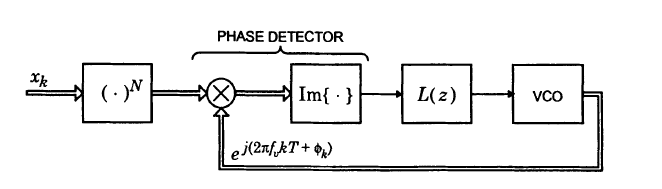
\includegraphics[width=0.7\columnwidth]{figs/powerN}
		\end{figure}
		
		\item Para demodular o sinal a senóide com frequência $N f_c$ deve ser convertida em outra com frequência $f_c$ utilizando um sintetizador.
		
		\item Embora não se encontre $N$ tal qual $e^{jN \phase A_k}=1$. A linha espectral em $N f_c$ ocorrerá se $E[A_k^N] \neq 0$.
		
	\end{itemize}
	
\end{frame}


